\documentclass{article}
\usepackage[utf8]{inputenc}
\usepackage{graphicx}
\usepackage{float}
\usepackage[danish]{babel}
\usepackage{hyperref}
\usepackage{amsmath}
\usepackage[]{algorithm2e}

\title{POP 2i - F\#}
\author{Sebastian Winkelmann (pbf475)}
\date{\today}

\begin{document}
\maketitle
\section*{2i.0 -- Konverteringstabel}
\begin{table}[H]
\centering
\begin{tabular}{|c|c|c|c|}
\hline
Decimal & Binær & Hexadecimal & Oktal \\ \hline
\textbf{10} & 1010 & a & 12 \\ \hline
21 & \textbf{10101} & 15 & 25 \\ \hline
63 & 111111 & \textbf{3f} & 77 \\ \hline
59 & 111011 & 3b & \textbf{73} \\ \hline
\end{tabular}
\caption{Udfyldt tabel med udregnede værdier for base $2$, $8$, $10$ og $16$}
\end{table}
\subsection*{Decimal til binær}
\begin{align*}
    \text{rest} & \leftarrow \text{værdi } \%\, 2\\
    \text{værdi} & \leftarrow \text{værdi}\, /\, 2\\
\end{align*}
Strengen som udgør det binære tal bliver herefter manipuleret, og rest indsættes i starten af strengen for hver cyklus: $$\text{binær}\leftarrow\text{rest}+\text{værdi}$$
\subsubsection*{$10_{10}$ til base 2}
\begin{align*}
    \text{rest}_0&=10\%2=0\\
    \text{værdi}_0&=10/2=5\\
    \text{rest}_1&=5\%2=1\\
    \text{værdi}_1&=5/2=2\\
    \text{rest}_2&=2\%2=0\\
    \text{værdi}_2&=2/2=1\\
    \text{rest}_3&=1\%2=1\\
    \text{værdi}_3&=1/2=0\\
\end{align*}
Vi konkatenerer hermed alle rest som strenge, startende fra (se bort fra kommutativitet, men bemærk at $n\geq0$, hvorfor summationen går baglæns) $i=n\to0$:$$\sum_{i=n}^{0}\text{rest}_i=\text{rest}_n+\cdots+\text{rest}_1+\text{rest}_0$$I dette tilfælde er $n=3$:\begin{equation}
    10_{10}\rightarrow1010_2
\end{equation}
Denne operationssekvens holder for alle tal. Det er derfor ikke nødvendigt at gøre det for alle base 10.
\subsection*{Decimal til hexadecimal}
I hexadecimal er der 16 forskellige værdier:$$\left\{0,1,2,3,4,5,6,7,8,9,a,b,c,d,e,f\right\}$$som hver især har en værdi repræsenteret ved der positionsindex -- altså $a\rightarrow10$, $b\rightarrow11$, $c\rightarrow12$, $d\rightarrow13$, $e\rightarrow14$ og $f\rightarrow15$. Vi bruger samme fremgangsmåde som med base 2, blot med 16 som divisor. Hermed:
\begin{align*}
    \text{rest} & \leftarrow \text{værdi } \%\, 16\\
    \text{værdi} & \leftarrow \text{værdi}\, /\, 16\\
\end{align*}
\subsubsection*{$10_{10}$ til base 16}
Da 10 ikke er delelig med 16, vil der kun være en rest:
\begin{align*}
    \text{rest}_0 & \leftarrow 10 \,\%\, 16=10
\end{align*}
Altså har vi at \begin{equation}
    10_{10}\rightarrow a_{16}
\end{equation}
\subsubsection*{$63_{10}$ til base 16}
Vi prøver med algoritmen:
\begin{align*}
    \text{rest}_0 & \leftarrow 63\, \%\, 16=15\\
    \text{værdi}_1 & \leftarrow 63\, /\, 16=3\\
\end{align*}
Vi har altså en kvotient og en rest (husk at $15\rightarrow f$). Dette sætter vi sammen:\begin{equation}
    63_{10}\rightarrow 3f_{16}
\end{equation}

\subsection*{Decimal til oktal}
Vi bruger samme fremgangsmåde som med base 2, blot med 8 som divisor. Hermed:
\begin{align*}
    \text{rest} & \leftarrow \text{værdi } \%\, 8\\
    \text{værdi} & \leftarrow \text{værdi}\, /\, 8\\
\end{align*}
\subsubsection*{$10_{10}$ til base 8}
Vi prøver med algoritmen:
\begin{align*}
    \text{rest}_0 & \leftarrow 10\, \%\, 8=2\\
    \text{værdi}_1 & \leftarrow 10\, /\, 8=1\\
\end{align*}
Vi har altså en kvotient og en rest. Dette sætter vi sammen:\begin{equation}
    10_{10}\rightarrow12_8
\end{equation}
\subsection*{Base 2, 8, 16 til base 10}
Jeg har i min besvarelse udelukkende konverteret værdier mellem base $n$ og 10 (decimal).
\subsubsection*{Fra binær til decimal}
For at finde decimalværdien af et binært tal tager vi det bageste bit, og ganger dets værdi med $2^0$, så det næste og ganger det med $2^1$:\begin{equation}
    x_{10}\rightarrow b_0\cdot2^0+b_1\cdot2^1+\cdots+b_n\cdot2^n\label{eq:add}
\end{equation}
\textbf{$10101_2$ til base 10}: Så vi bruger bare (\ref{eq:add}):\begin{align*}
    10101_2&\rightarrow 1\cdot2^0+0\cdot1^1+1\cdot2^2+0\cdot2^3+1\cdot2^4\\
    10101_2&\rightarrow 21_10
\end{align*}
\textbf{$111011_2$ til base 10}: Så vi bruger bare (\ref{eq:add}):\begin{align*}
    111011_2&\rightarrow 1\cdot2^0+1\cdot2^1+0\cdot2^2+1\cdot2^3+1\cdot2^4+1\cdot2^5\\
    111011_2&\rightarrow 59_10
\end{align*}
\subsubsection*{Fra hexadecimal til decimal}
For at finde decimalværdien af hexadecimaler tager vi det bageste ciffer og ganger dets værdi med $16^0$, så det næste og ganger det med $16^1$:\begin{equation}
    x_{10}\rightarrow h_0\cdot16^0+h_1\cdot16^1+\cdots+h_n\cdot16^n\label{eq:addhex}
\end{equation}
\textbf{$3\text{f}_{16}$ til base 10}: Så vi bruger bare (\ref{eq:addhex}):\begin{align*}
    3f_{16}&\rightarrow f\cdot16^0+3\cdot16^1\\
    3f_{16}&\rightarrow 15\cdot16^0+3\cdot16^1\\
    3f_{16}&\rightarrow 63_{10}
\end{align*}
\subsubsection*{Fra oktal til decimal}
For at finde decimalværdien af hexadecimaler tager vi det bageste ciffer og ganger dets værdi med $8^0$, så det næste og ganger det med $8^1$:\begin{equation}
    x_{10}\rightarrow o_0\cdot8^0+o_1\cdot8^1+\cdots+o_n\cdot8^n\label{eq:addok}
\end{equation}
\textbf{$78_8$ til base 10}: Så vi bruger bare (\ref{eq:addok}):\begin{align*}
    73_8&\rightarrow 3\cdot8^0+7\cdot8^1\\
    73_8&\rightarrow 3+56\\
    73_8&\rightarrow 59_{10}
\end{align*}
\subsection{Kode}
For at finde alle værdierne har jeg lavet et lille program i F\#. Den kører alle ovenstående funktioner.
\section*{2i.1 -- Beskrivelse af \textbackslash n}
Udtrykket \texttt{"hello\textbackslash nworld\textbackslash n"} laver en string:\begin{verbatim}
    "hello
    world
    "
\end{verbatim}
Hvor \texttt{\textbackslash n} blot laver en ny linje, da det er escape-sequence som betyder \textit{new line}. Resultatet er rigtignok "hello world" blot med ny linje efter \textit{hello} og \textit{world}. 
\section*{2i.2 -- Escape}
Ved at bruge en verbatim-streng kan man undgå at escape-udtryk virker i strengen. Enten ved \texttt{@"\textbackslash n"} eller \texttt{"{}"{}"{}\textbackslash n"{}"{}"}. Disse to strengmiljøer er til for at man kan skrive mere frit, samt lave afstand uden brug af escape-sequences.
\begin{figure}[H]
    \centering
    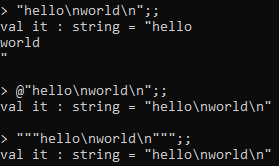
\includegraphics[width=0.5\textwidth]{cmd_dHJkJPD6Jk.png}
    \caption{Tre forskellige strengmiljøer med escape-sequences}
    \label{fig:escapeenv}
\end{figure}
\section*{2i.3 -- Strengindicering}
Lad os først definere strengen, og herefter benytte indicering på strengen for de første 5 bogstaver, og dernæst de sidste 5 bogstaver (når \texttt{streng.Length = 11}):\begin{verbatim}
    val streng = "hello world"
    val a = streng.[0..4]
    val b = streng.[6..10]
\end{verbatim}
Se figur \ref{fig:stringindex} for kode og resultat i \texttt{fsharpi}.
\begin{figure}[H]
    \centering
    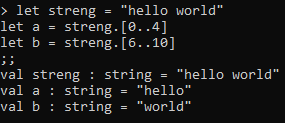
\includegraphics[width=0.5\textwidth]{cmd_VlnBcCJX7c.png}
    \caption{Seperation af streng vha. indicering}
    \label{fig:stringindex}
\end{figure}
\end{document}